\selectlanguage{english}

\chapter{Reject Inference} \label{chap2}

\epigraph{Sounds good, doesn't work.}{Donald J.\ Trump}

\minitoc

%\textit{Nota Bene :} ce chapitre s'inspire fortement de l'article [...]

\bigskip

The granting process of all credit institutions in based on the probability that the applicant will refund his loan given his characteristics. This probability also called \gls{score} is learnt based on a dataset in which rejected applicants are \textit{de facto} excluded. This implies that the population on which the score is used will be different from the learning population. Thus, this biased learning can have consequences on the scorecard relevance. Many methods in the field of reject inference have been developed in order to try to exploit the data available from the rejected applicants to build the score. However most of these methods are considered from an empirical point of view, and there is some lack of formalisation of the assumptions that are really made, and of the theoretical properties that can be expected. We propose a formalisation of these usually hidden assumptions for some of the most common reject inference methods, and we discus the improvement that can be expected. These conclusions are illustrated on simulated data and on real data from the French branch of Crédit Agricole Consumer Finance (CA CF).


\section{Introduction}


In consumer loans, the acceptance process was described in Chapter~\ref{chap1} and can be formalized as follows. For a new applicant's profile and credit's characteristics, the lender aims at estimating the repayment probability. To this end, the \textit{credit modeler} fits a predictive model, often a \gls{lr}, between already  financed  clients' characteristics $\glssymbol{bx}=(\glssymbol{x}_1,\ldots,\glssymbol{x}_d)$ and their repayment status, a binary variable $\glssymbol{y}\in\{0,1\}$ (where $1$ corresponds to good clients and $0$ to bad clients). The model is then applied to the new applicant and yields an estimate of its repayment probability. In practice, an increasing transformation of this probability also called score is often considered.
Under some cut-off value of the \gls{score} (see Section~\ref{subsec:critere}) the applicant is rejected, except if further expert rules come into play as can be seen from Figure~\ref{fig:figure1}.

\begin{figure}[ht]
\begin{minipage}[b]{0.45\linewidth}
\center \includegraphics[width=5cm]{figures/chapitre2/schema.png}
\caption{Simplified Acceptance mechanism in~Crédit Agricole Consumer Finance}
\label{fig:figure1}

\end{minipage}%
\hfil \begin{minipage}[b]{0.5\linewidth}

\center 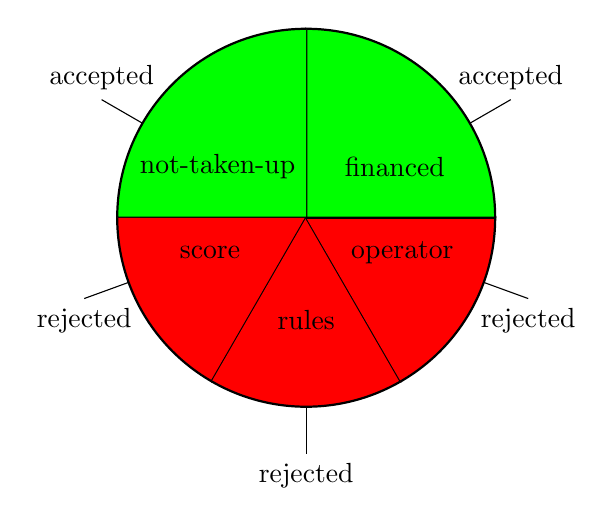
\begin{tikzpicture}

    \foreach \start/\end/\middle/\percent/\anchor/\name in {
      0/90/30/financed/above/accepted,
      90/180/150/not-taken-up/above/accepted}
  {
    \draw[fill=green, thick] (0,0) -- (\end:2.4cm) arc (\end:\start:2.4cm)
      node at (\middle:1.3cm) {\percent};
    \draw (\middle:2.4cm) -- (\middle:3cm) node[\anchor] {\name};
  };
    
    \foreach \start/\end/\middle/\percent/\anchor/\name in {
      180/240/200/score/below/rejected,
      240/300/270/rules/below/rejected,
      300/360/340/operator/below/rejected}
  {
    \draw[fill=red, thick] (0,0) -- (\end:2.4cm) arc (\end:\start:2.4cm)
      node at (\middle:1.3cm) {\percent};
    \draw (\middle:2.4cm) -- (\middle:3cm) node[\anchor] {\name};
  };
\end{tikzpicture}
\caption{Simplified Acceptance status in Crédit Agricole Consumer Finance - scale relations not respected}
\label{fig:figure2}

\end{minipage}
\end{figure}
 


The through-the-door population (all applicants) can be classified into two categories thanks to a binary variable $z$ taking values in $\{\f,\nf\}$ where $\f$ stands for financed applicants (in \textcolor{green}{green} on FIgure~\ref{fig:figure2}) and $\nf$ for not financed ones (in \textcolor{red}{red} on FIgure~\ref{fig:figure2}). As the repayment variable $\glssymbol{y}$ is unobserved for not financed applicants, credit scorecards are only constructed on financed clients' data but then applied to the whole  through-the-door population. The relevance of this process is a natural question which is dealt in the field of \textit{reject inference}. The idea is to use the characteristics of not financed clients in the scorecard building process to avoid a population bias, and thus to improve the prediction on the whole through-the-door population. Such methods have been described in~\cite{RI6,saporta,banasik,economix}, and have also notably been investigated in~\cite{RI2} who first saw \textit{reject inference} as a missing data problem. In~\cite{RI3}, the misspecified model case on real data is studied specifically and is also developed here.


In fact, it can be considered as a part of the semi-supervised learning setting, which consist in learning from both labelled and unlabelled data. However, in the semi-supervised setting~(\cite{ChaSchZie06}) it is generally assumed that labelled data and unlabelled data come from the same distribution, which is rarely the case in \textit{Credit Scoring}. Moreover, the main case of use of semi-supervised learning is when the number of unlabelled data is far larger than the number of labelled data, which is not the case in \textit{Credit Scoring} since the number of rejected clients and accepted clients is often balanced and depends heavily on the financial institution, the portfolio considered, etc.


The purpose of the present chapter is twofold: a clarification of which mathematical hypotheses, if any, underlie those reject inference methods and a clear conclusion on their relevance. In Section~\ref{sec:criteres}, we present a criterion to assess a method's performance and discuss missingness mechanisms that characterize the relationship of $\glssymbol{z}$ with respect to $\glssymbol{bx}$ and $\glssymbol{y}$. In Section~\ref{sec:methods_reject}, we go through some of the most common reject inference methods and exhibit their mathematical properties. Finally, to confirm our theoretical findings, we test each method on simulated and real data from Crédit Agricole Consumer Finance in Section~\ref{sec:experiments}.

\textcolor{blue}{CB : ajouter description partie 5 (conclusion)}

\section{\textit{Credit Scoring} modelling} \label{sec:criteres}

\subsection{Data} 

The decision process of financial institutions to accept a credit application is usually embedded in the  probabilistic framework. This latter offers rigorous tools for taking into account both variability of applicants and uncertainty on their ability to pay back the loan. In this context, the important term is $p(\glssymbol{y}|\glssymbol{bx})$, designing the probability that a new applicant (described by his characteristics $\glssymbol{bx}$) will pay back his loan ($\glssymbol{y}=1$) or not ($\glssymbol{y}=0$). Estimation of $p(\glssymbol{y}|\glssymbol{bx})$ is thus an essential task of any credit scoring process.

For performing estimation, a specific $n$-sample $\mathcal{T}$ is available, decomposed into two disjoints and meaningful subsets, denoted by $\mathcal{T}_{\text{f}}$ and $\mathcal{T}_{\text{nf}}$ ($\mathcal{T}=\mathcal{T}_{\text{f}} \sqcup \mathcal{T}_{\text{nf}} \equiv \mathcal{T}=\mathcal{T}_{\text{f}} \cup \mathcal{T}_{\text{nf}}$, $\mathcal{T}_{\text{f}}\cap \mathcal{T}_{\text{nf}}=\emptyset$). The first subset ($\mathcal{T}_{\text{f}}$) corresponds to applicants with features $\glssymbol{bx}_i$ who have been financed ($\glssymbol{z}_i={\text{f}}$) and, consequently, for who the repayment status $\glssymbol{y}_i$ is known. Thus, $\mathcal{T}_{\text{f}}=(\glssymbol{bx}_i,\glssymbol{y}_i,\glssymbol{z}_i)_{i\in \text{F}}$ where $\text{F}=\{i:\glssymbol{z}_i={\text{f}}\}$ denotes the corresponding subset of indexes. The second subset ($\mathcal{T}_{\text{nf}}$) corresponds to applicants with features $\glssymbol{bx}_i$ who have {\it not} been financed ($\glssymbol{z}_i={\text{nf}}$) and, consequently, for who the repayment status $\glssymbol{y}_i$ is {\it unknown}. Thus, $\mathcal{T}_{\text{nf}}=(\glssymbol{bx}_i,\glssymbol{z}_i)_{i\in \text{NF}}$ where $\text{NF}=\{i:z_i={\text{nf}}\}$ denotes the corresponding subset of indexes. We notice that $\glssymbol{y}_i$ values are excluded from the observed sample $\mathcal{T}_{\text{nf}}$, since they are missing. These data can be represented schematically as:

\[ \mathcal{T} = \begin{array}{c}
\mathcal{T}_{\text{f}} = ( \tikzmarkin[hor=style green]{el02} \bm{x}^{\text{f}} \tikzmarkend{el02}\\
\\
\sqcup \\
\\
\mathcal{T}_{\text{nf}} = ( \tikzmarkin[hor=style orange]{el-12} \bm{x}^{\text{nf}} \tikzmarkend{el-12} \end{array}
\left( \begin{array}{ccc}
%\rowcolor{red!20}
\tikzmarkin[hor=style green]{e1} \; \; x_1^1 & \cdots & x_1^d  \\
 \vdots & \vdots & \vdots  \\
 x_n^1 & \cdots & x_n^d \tikzmarkend{e1} \\
\tikzmarkin[hor=style orange]{e2} \; \; x_{n+1}^1 & \cdots & x_{n+1}^d  \\
 \vdots & \vdots & \vdots \\
 x_{n+m}^1 & \cdots & x_{n+m}^d \tikzmarkend{e2} \end{array} \right),
 \hspace{1.5cm}
 \begin{array}{c}
\tikzmarkin[hor=style green]{el11} \bm{y}^{\text{f}} \tikzmarkend{el11}\\
\\
\\
\\
\tikzmarkin[hor=style orange]{el12} \bm{y}^{\text{nf}} \tikzmarkend{el12}\end{array}
\left( \begin{array}{c}
\tikzmarkin[hor=style green]{e4} y_1 \\
\vdots \\
y_n \tikzmarkend{e4} \\ 
\tikzmarkin[hor=style orange]{e3} \text{NA} \\
\vdots \\
\text{NA} \tikzmarkend{e3} \end{array} \right) ,
 \hspace{1.5cm}
 \begin{array}{c}
\tikzmarkin[hor=style green]{el111} \bm{z}^{\text{f}} \tikzmarkend{el111}\\
\\
\\
\\
\tikzmarkin[hor=style orange]{el121} \bm{z}^{\text{nf}} \tikzmarkend{el121}\end{array}
\left( \begin{array}{c}
\tikzmarkin[hor=style green]{e41} \text{f} \\
\vdots \\
\text{f} \tikzmarkend{e41} \\ 
\tikzmarkin[hor=style orange]{e31} \text{nf} \\
\vdots \\
\text{nf} \tikzmarkend{e31} \end{array} \right)
 \hspace{0.2cm}
 \begin{array}{c}
). \\
\\
\\
). \end{array}
\]


\subsection{General parametric model}

Estimation of $p(\glssymbol{y}|\glssymbol{bx})$ has to rely on modelling since the true probability distribution it is unknown. Firstly, it is both convenient and realistic to assume that triplets $(\glssymbol{bx}_i,\glssymbol{y}_i,\glssymbol{z}_i)_{1\le i\le n}$ are all independent and identically distributed (i.i.d.), including the unknown values of $\glssymbol{y}_i$ when $i\in \text{NF}$. Secondly, it is usual and convenient to assume that the unknown distribution $p(y|x)$ belongs to a given parametric family $\{p_{\glssymbol{bth}}(\glssymbol{y}|\glssymbol{bx})\}_{\glssymbol{bth} \in\Theta}$, where $\Theta$ is the parameter space as was discussed in Chapter~\ref{chap1}. For instance, \gls{lr} is often considered in practice, even if we will be more general in this section. However, \gls{lr} will be important for other sections since some standard reject inference methods are specific to this family (Section~\ref{sec:methods_reject}) and numerical experiments (Section~\ref{sec:experiments_reject}) will implement them.

As in any missing data situation (here $\glssymbol{z}$ indicates if $\glssymbol{y}$ is missing or not), the relative modelling process, namely $p(\glssymbol{z}|\glssymbol{bx},\glssymbol{y})$, has also to be clarified. For convenience, we can also consider a parametric family $\{p_{\glssymbol{phi}}(\glssymbol{z}|\glssymbol{bx},\glssymbol{y})\}_{\glssymbol{phi} \in \Phi}$, where $\glssymbol{phi}$ denotes the parameter and $\Phi$ the associated parameter space. Note we consider here the most general missing data situation, namely a \glsfirst{mnar} mechanism. It means that $\glssymbol{z}$ can be stochastically dependent on some missing data $\glssymbol{y}$, namely that $p(\glssymbol{z}|\glssymbol{bx},\glssymbol{y})\neq p(\glssymbol{z}|\glssymbol{bx})$. We will discuss this fact in Section~\ref{sec:mechanisms}.

Finally, combining both previous distributions $p_{\glssymbol{bth}}(\glssymbol{y}|\glssymbol{bx})$ and $p_{\glssymbol{phi}}(\glssymbol{z}|\glssymbol{bx},\glssymbol{y})$ leads to express the joint distribution of $(\glssymbol{y},\glssymbol{z})$ conditionally to $\glssymbol{bx}$ as:
\begin{equation}\label{eq:generative}
p_{\gamma}(\glssymbol{y},\glssymbol{z}|\glssymbol{bx}) = p_{\glssymbol{phi}(\gamma)}(\glssymbol{z}|\glssymbol{y},\glssymbol{bx})p_{\glssymbol{bth}(\gamma)}(\glssymbol{y}|\glssymbol{bx}).
\end{equation}
where $\{p_{\gamma}(\glssymbol{y},\glssymbol{z}|\glssymbol{bx})\}_{\gamma \in \Gamma}$ denotes a distribution family indexed by a parameter $\gamma$ evolving in a space $\Gamma$. Here it is clearly expressed that both parameters $\glssymbol{phi}$ and $\glssymbol{bth}$ depend on $\gamma$, even if in the following we will note shortly $\glssymbol{phi}=\glssymbol{phi}(\gamma)$ and $\glssymbol{bth}=\glssymbol{bth}(\gamma)$. In the most general missing data situation, the missing process is said to be {\it non-ignorable}, meaning that parameters $\glssymbol{phi}$ and $\glssymbol{bth}$ can be functionality dependent (thus $\gamma\neq (\glssymbol{phi},\glssymbol{bth})$). We also discuss this fact in Section~\ref{sec:mechanisms}.

\subsection{Maximum likelihood estimation} 
\label{sec:EM}

Mixing previous model and data, the maximum likelihood principle can be invoked for estimating the whole parameter $\gamma$, thus yielding as a by-product the parameter $\glssymbol{bth}$. Indeed, $\glssymbol{bth}$ is of particular interest, the goal of the financial institutions being solely to obtain an estimate of $p_{\glssymbol{bth}}(\glssymbol{y}|\glssymbol{bx})$. The observed log-likelihood can be written as:
\begin{equation}\label{eq:like.MNAR}
\ell(\gamma;\mathcal{T}) = \sum_{i\in\text{F}}\ln p_{\gamma}(\glssymbol{y}_i,\text{f} | \glssymbol{bx}_i) + \sum_{i'\in\text{NF}} \ln \left[ \sum_{\glssymbol{y}\in\{0,1\}} p_{\gamma}(\glssymbol{y},\text{nf} | \glssymbol{bx}_{i'}) \right].
\end{equation}
Within this missing data paradigm, the EM algorithm (see~\cite{dempster1977maximum}) can be used. Starting from an initial value $\gamma^{(0)}$, iteration $(s)$ of the algorithm is decomposed into the following two classical steps:
\paragraph{E-step} compute the conditional probabilities of missing $\glssymbol{y}_i$ values:
\begin{equation}
t_{i\glssymbol{y}}^{(s)} = p_{\glssymbol{bth}(\gamma^{(s-1)})}(\glssymbol{y}|\glssymbol{bx}_i,\nf) = \frac{p_{\gamma^{(s-1)}}(\glssymbol{y}, \nf|\glssymbol{bx}_i)}{\sum_{\glssymbol{y}' = 0}^{1} p_{\gamma^{(s-1)}}(\glssymbol{y}', \nf|\glssymbol{bx}_i)};
\end{equation}
\paragraph{M-step} maximize the conditional expectation of the complete log-likelihood:
\begin{equation}\label{eq:like.c}
\ell_c(\gamma;\mathcal{T}_c) = \sum_{i=1}^n\ln p_{\gamma}(\glssymbol{y}_i,\glssymbol{z}_i | \glssymbol{bx}_i)
\end{equation}
leading to:
\begin{equation}
\gamma^{(s)} = \argmax_{\gamma \in \Gamma} \sum_{i\in \text{F}} \ln p_{\gamma}(\glssymbol{y}_i, \f|\glssymbol{bx}_i) +  \sum_{i'\in \text{NF}}\sum_{\glssymbol{y} = 0}^{1}t_{i'\glssymbol{y}}^{(s)} \ln p_{\gamma}(\glssymbol{y}, \nf | \glssymbol{bx}_{i'}).
\end{equation}
Usually, stopping rules rely either on a predefined iteration number, or on a predefined stability criterion of the observed likelihood.

\subsection{Some current restrictive missingness mechanisms}
\label{sec:mechanisms}

The latter parametric family is very general since it considers both that the missingness mechanism is \gls{mnar} and non-ignorable. But in practice, it is commo, to consider ignorable models for the sake of simplicity, meaning that $\gamma= (\glssymbol{phi},\glssymbol{bth})$. There exists also some restrictions to the \gls{mnar} mechanism. 

The first restriction to \gls{mnar} is the\glsfirst{mcar} setting, meaning that $p(\glssymbol{z}| \glssymbol{bx},\glssymbol{y}) = p(\glssymbol{z})$. In that case, applicants should be accepted or rejected without taking into account their descriptors $\glssymbol{bx}$. Such a process is not realistic at all for representing the actual process followed by financial institutions. Consequently it is always discarded in \textit{Credit Scoring}.

The second restriction to \gls{mnar} is the \glsfirst{mar} setting, meaning that $p(\glssymbol{z}| \glssymbol{bx},\glssymbol{y}) = p(\glssymbol{z}|\glssymbol{bx})$. The \gls{mar} missingness mechanism seems realistic for \textit{Credit Scoring} applications, for example when the financing is based solely on a function of $x$, {\it e.g.} in the case of a score associated to a cut-off. It is a usual assumption in credit scoring even if, in practice, the financing mechanism may depend also on unobserved features (thus not present in $\glssymbol{bx}$). In the \gls{mar} situation the log-likelihood~(\ref{eq:like.MNAR}) can be reduced to:
\begin{equation}\label{eq:like.MAR}
\ell(\gamma;\mathcal{T}) = \ell(\glssymbol{bth};\mathcal{T}_{\text{f}}) + \sum_{i'=1}^n \ln p_{\glssymbol{phi}}(\glssymbol{z}_{i'} | \glssymbol{bx}_{i'}),
\end{equation}
with $\ell(\glssymbol{bth};\mathcal{T}_{\text{f}})=\sum_{i\in\text{F}}\ln p_{\glssymbol{bth}}(\glssymbol{y}_i | \glssymbol{bx}_i)$.
Combining it with the ignorable assumption, estimation of $\glssymbol{bth}$ relies only on the first part $\ell(\glssymbol{bth};\mathcal{T}_{\text{f}})$, since the value $\glssymbol{phi}$ has no influence on~$\glssymbol{bth}$. In that case, invoking an EM algorithm due to missing data $\glssymbol{y}$ is no longer required as will be made explicit in Section~\ref{subsec:no_reject}.

\subsection{Model selection}

At this step, several kinds of parametric model~(\ref{eq:generative}) have been assumed. It concerns obviously the parametric family $\{p_{\glssymbol{bth}}(\glssymbol{y}|\glssymbol{bx})\}_{\glssymbol{bth} \in\Theta}$, and also the missingness mechanism \gls{mar} or \gls{mnar}. 
However, it has to be noticed that \gls{mar} versus \gls{mnar} cannot be tested since we do not have access to $\glssymbol{y}$ for not financed clients~\cite{molenberghs2008every}. However, model selection is possible by modelling also the whole financing mechanism, namely the family $\{p_{\glssymbol{phi}}(\glssymbol{z}|\glssymbol{bx},\glssymbol{y})\}_{\glssymbol{phi} \in \Phi}$.


Scoring for credit application can be recast as a semi-supervised classification problem \textcolor{blue}{ref chapel}. In this case, classical model selection criteria can be divided into two categories \textcolor{blue}{ref these VV}: either scoring performance criteria as \textit{e.g.}\ error rate on a test set, or information criteria as \textit{e.g.}\ BIC as was introduced in Section~\ref{subsubsec:choix_modele}.

In the category of error rate criteria, the typical error rate is expressed as follows:
\begin{equation}
\mbox{error} = \frac{1}{m} \sum_{i=n+1}^{n+m} \mathbb{I}(\hat y_i \neq y_i),
\end{equation} 
where $(y_{n+1},\ldots,y_{n+m})$ is a $m$-sample (test sample) i.i.d. from $p(\glssymbol{y}|\glssymbol{bx})$ and where $\hat{\glssymbol{y}}_i$ is the estimated value of the related $\glssymbol{y}_i$ value involved by the estimated model at hand. The model leading to the lowest error value is then retained. However, in the credit scoring context this criterion family is not available since no sample $(y_{n+1},\ldots,y_{n+m})$ is itself available. This problem can be seen through the following straightforward expression
\begin{equation}\label{eq:error}
p(\glssymbol{y}|\glssymbol{bx}) = \sum_{\glssymbol{z}\in\{\text{f},\text{nf}\}} p(\glssymbol{y}|\glssymbol{bx},\glssymbol{z}) p(\glssymbol{z}|\glssymbol{bx})
\end{equation}
where $p(\glssymbol{y}|\glssymbol{bx},\glssymbol{z})$ is unknown and $p(\glssymbol{z}|\glssymbol{bx})$ is known since this latter is defined by the financial institution itself. We notice that obtaining a sample from $p(\glssymbol{y}|\glssymbol{bx})$ would require that the financial institution draws $(\glssymbol{z}_{n+1},\ldots,\glssymbol{z}_{n+m})$ i.i.d. from $p(\glssymbol{z}|\glssymbol{bx})$ before to observe the results $(\glssymbol{y}_{n+1},\ldots,\glssymbol{y}_{n+m})$ i.i.d. from $p(\glssymbol{y}|\glssymbol{bx},\glssymbol{z})$. But in practice it is obviously not the case, a threshold being applied to the distribution $p(\glssymbol{z}|\glssymbol{bx})$ for retaining only a set of fundable applicants, the non-fundable applicants being definitively discarded. As a matter of fact, only a sample of $p(\glssymbol{y}|\glssymbol{bx},\text{f})$ is available, 
irrevocably prohibiting the calculus of~(\ref{eq:error}) as a model selection criterion.

In the category of information criteria, the BIC criterion (presented in Section~\ref{subsubsec:choix_modele}) is expressed as the following penalization of the maximum log-likelihood:
\begin{equation}\label{eq:AIC}
\mbox{BIC} = 2 \ell(\hat\gamma;\mathcal{T}) - |\Gamma| \ln n,
\end{equation}
where $\hat\gamma$ is the maximum likelihood estimate of $\gamma$ and $|\Gamma|$ is the number of parameters to be estimated in the model at hand. The model leading to the greatest BIC value is then retained. Many other BIC-like criteria exist \textcolor{blue}{ref these VV} but the underlined idea is unchanged. Contrary to the error rate criteria like~(\ref{eq:error}), it is thus possible to compare models without funding ``non-fundable applicants'' since just the available sample $\mathcal{T}$ is required. However, computing~(\ref{eq:AIC}) requires to precisely express the model families $\{p_{\gamma}(\glssymbol{y},\glssymbol{z}|\glssymbol{bx})\}_{\gamma \in Gamma}$ which compete.

\section{Rational reinterpretation of \textit{reject inference} methods} \label{sec:methods_reject}

\subsection{The reject inference challenge}

As discussed in the previous section, a regular way to use the whole observed sample $\mathcal{T}$ in the estimation process implies some challenging modeling and assumptions steps. A method using the whole sample $\mathcal{T}$ is traditionally called a {\it rejection inference} method since it uses not only financed applicants (sample $\mathcal{T}_\text{f}$) but also not financed, or rejected, applicants (sample $\mathcal{T}_{\text{nf}}$).
Since modeling is sometimes a too heavy task, some methods propose alternatively to involve the whole sample $\mathcal{T}$ in a more empirical manner. However, this is somewhere a risky strategy since we have also seen in the previous section that validating methods with error rate like criteria is not possible through the standard credit scoring process. As a result, some strategies are proposed to perform a ``good'' \gls{score} function estimation without possibility to access its real performance.

However, most of the proposed reject inference strategies may make some hidden assumptions on the modeling process. Our challenge is to reveal as far as possible such hidden assumptions to then discuss their realism,  
failing to be able to compare them by the model selection principle.

\subsection{Strategy 1: ignoring not financed clients} \label{subsec:no_reject}

\subsubsection{Definition}
The simplest reject inference strategy is to ignore not financed clients for estimating $\glssymbol{bth}$. Thus it consists to estimate $\glssymbol{bth}$ by maximizing the log-likelihood $\ell(\glssymbol{bth};\mathcal{T}_{\text{f}})$.

\subsubsection{Interpretation}
In fact, this strategy is equivalent to using the whole sample $\mathcal{T}$ (financed and not financed applicants) under both the \gls{mar} and ignorable assumptions. See the related explanation in Section~\ref{sec:mechanisms}. Consequently, this strategy is truly a particular ``reject inference'' strategy although it does not seem to be.

\subsection{Strategy 2: reclassification}

\subsubsection{Definition}
This strategy corresponds to an algorithm which is starting with $\theta^{(0)}$ the value which maximizes the log-likelihood $\ell(\glssymbol{bth};\mathcal{T}_{\text{f}})$ restricted to the financed client. Then, all $(\glssymbol{y}_i)^{(1)}_{i \in \nf}$ are imputed by the {\it maximum a posteriori} (MAP) principle given by: $\hat{\glssymbol{y}}^{(1)}_i = \argmax_{\glssymbol{y} \in \{0,1\}} p_{\hat{\glssymbol{bth}^{(0)}}_{\text{f}}}(\glssymbol{y} | \glssymbol{bx}_i)$. The completed log-likelihood $\ell_c(\glssymbol{bth};\mathcal{T}_c^{(1)})$ given in~(\ref{eq:like.c}) and with $\mathcal{T}_c^{(1)}=\mathcal{T} \cup (\glssymbol{y}_i)^{(1)}_{i \in \nf}$ is maximized and yields parameter estimate $\hat{\glssymbol{bth}}^{(1)}$. Its first variant stops at this value $\hat{\glssymbol{bth}}^{(1)}$. Its second variant iterates until potential convergence of $(\hat{\glssymbol{bth}}^{(s)})$, $s$ designing the iteration number. In practice, this method can be found in~\cite{saporta} under the name ``iterative reclassification'' in~\cite{RI6}  under the name ``reclassification'' or under the name ``extrapolation'' in~\cite{banasik}. The completed data can be expressed schematically as:

\[ \mathcal{T}_c = \begin{array}{c}
\tikzmarkin[hor=style green]{el0} \bm{x}^{\text{f}} \tikzmarkend{el0} \\
\\
\\
\tikzmarkin[hor=style green]{el-1} \bm{x}^{\text{nf}} \tikzmarkend{el-1} \end{array}
\left( \begin{array}{ccc}
%\rowcolor{red!20}
\tikzmarkin[hor=style green]{el1} \; \; x_1^1 & \cdots & x_1^d  \\
 \vdots & \vdots & \vdots \\
 x_n^1 & \cdots & x_n^d \\
 x_{n+1}^1 & \cdots & x_{n+1}^d  \\
 \vdots & \vdots & \vdots \\
 x_{n+m}^1 & \cdots & x_{n+m}^d \tikzmarkend{el1} \end{array} \right)
 \begin{array}{c}
\tikzmarkin[hor=style green]{l1} \bm{y}^{\text{f}} \tikzmarkend{l1}\\
\\
\\
\tikzmarkin[hor=style green]{l2} \bm{y}^{\text{nf}} \tikzmarkend{l2} \end{array}
\left( \begin{array}{c}
\tikzmarkin[hor=style green]{l3} \; \; y_1 \; \; \; \\
\vdots \\
 y_n \\ 
 \hat{\glssymbol{y}}_{n+1} \\
\vdots \\
\hat{\glssymbol{y}}_{n+m} \tikzmarkend{l3}\end{array} \right)\]

\subsubsection{Interpretation}
This algorithm is equivalent to the so-called \gls{cem} algorithm where a Classification (or MAP) step is inserted between the Expectation and Maximization steps of an \gls{em} algorithm (described in Section~\ref{sec:EM}). It can be found in \cite{RI6}, also sometimes referred to as extrapolation as in \cite{banasik}. CEM aims at maximizing the completed log-likelihood $\ell_c(\glssymbol{bth};\mathcal{T}_c)$ over both $\glssymbol{bth}$ and $(\glssymbol{y}_i)_{i \in \nf}$. Since $\glssymbol{phi}$ is not involved in this process, we first deduce from Section~\ref{sec:mechanisms} that, again, \gls{mar} and ignorable assumptions are present. Then, standard properties of the estimate maximizing the completed likelihood indicate that it is not a consistent estimate of $\glssymbol{bth}$ \textcolor{blue}{ref}, contrary to the traditional maximum likelihood one, as can be seen from Figure~\ref{fig:biais_CEM}.


\begin{figure}[ht]
\center \includegraphics[width=\textwidth]{figures/chapitre2/CEM_bias.png}
\caption{In the context of a probabilistic classifier, it is known that the CEM algorithm employed implicitly by the Reclassification method amounts to a bigger bias in terms of \gls{lr} parameters, but a ``sharper'' decision boundary.}
\label{fig:biais_CEM}
\end{figure}





\section{Consumer loans: acceptance and financing process}




















\printbibliography[heading=subbibliography, title=References of Chapter 2]